\documentclass{article}

\usepackage[utf8]{inputenc}
\usepackage{graphicx} % Comandos para manejar imágenes
\graphicspath{ {./images/} } % Carpeta de imágenes

\setlength{\parskip}{2mm} % Espaciado

\usepackage[utf8]{inputenc}
\usepackage{geometry}
    \geometry{left=3cm,right=2cm,top=2cm,bottom=2cm}
%
\usepackage[spanish]{babel}
%
\usepackage[fixlanguage]{babelbib}
    \bibliographystyle{babunsrt}
%
\usepackage{url}

\usepackage[top=2cm, bottom=2.5cm, right=3 cm, left=3 cm]{geometry} % margenes

\usepackage{parskip} % Sangria

\title{Seminar one: Around the forecast of the Power System behavior, notes about the presentation of the professor Felipe Feijoo Palacios, PhD.}
\author{Cristóbal Galleguillos Ketterer$^{1}$\\
\small{$^{1}$Industrial PhD Program}\\
\small{Pontificia Universidad Católica de Valparaíso}\\
\small{cristobal.galleguillos@pucv.cl}
}
\date{\small{\today}}

\begin{document}

\maketitle

\section{Introduction}

The power system is the most complex and largest industrial system ever built, in simple terms is composed of four different sub systems:

\begin{itemize}
    \item Generation,
    \item Distribution,
    \item Transmission, and,
    \item Consumers,
\end{itemize}

Between the consumers is possible to differentiate free consumers and regulated consumers, according to the nature of the contractual with de generators or distributors.

\subsection{Scope}

This work is based in a partial of the presentation of the lecturer Felipe Feijoo, given in the framework of the Industrial PhD program of the Pontificia Universidad Católica de Valparaíso.

Focused on the work included in the paper named \textit{Design of Pareto optimal CO2 cap-and-trade policies for deregulated electricity networks}.

\section{Literature review}

The search in the specialized web ScienceDirect of the words "Power Marker" give 493,723 scientists articles, dedicated to the thematic of study.

We select more a less random, two documents that approach the phenomenon of energy from two points of view

\begin{itemize}
    \item As a chaotic and non-linear system
    \item As a complex system (energy-cyber-physical-systems  improve flexibility in fuel sources & energy products)
\end{itemize}

It is a constantly changing field, so there is no single paradigm. It is possible to find approaches more or less holistic or more or less based on classical mathematical methods.

In addition, is important basic theoretical formulation of the Game Theory included, for example in advanced microeconomics's textbook-like Varian, the demonstrations, theorems, and axioms exposing in this canonical text allow know if the main assumptions of the author are used adequately.

\section{Framework}


Mathematical resolution is function of the computational accesses, is possible whit a lot of time of super computing we resolve a more complex (or sophisticated) resolution of mathematical solver at problems whit the form

\begin{equation}
\textbf{[A][x]=[b]}\label{it}   
\end{equation}

When
\begin{itemize}
    \item \textbf{[A]} is a matrix of coefficients.
    \item \textbf{[x]} is a vector of unknowns, and.
    \item \textbf{[b]} is a vector of solutions.
\end{itemize}

In addition, the lecturer modeling the system like as simultaneous games (MPEC,EPEC).

\section{Author's Contribution}

The authors declare in their objective as contribution to the investigation the following: 

\begin{itemize}
    \item The model is a can serve as a useful tool for policy makers to select alternative (cap and trade) C&T policies satisfying various interests of the electricity net-work constituents. 
\end{itemize}

The impact of these policies can be verified in:

\begin{itemize}
    \item Higher consumption
    \item Lower emissions
    \item Lower electricity prices
\end{itemize}

Also, the results presented in the paper also examine:

\begin{itemize}
    \item The sensitivity of factors affecting electricity market
    \item Social cost of carbon
    \item demand-price sensitivity. 
\end{itemize}

\subsection{Something about metrics}

Just to get an idea about the particular impact of this article and the author, we present the main metrics indicated on the portal ScienceDirect, in the figure shown below:

\begin{figure}[h]
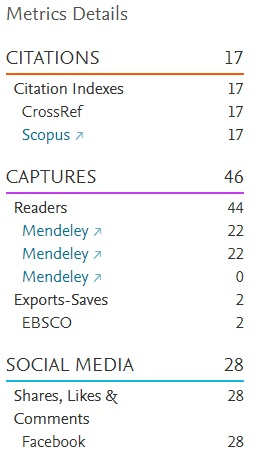
\includegraphics[scale=.5]{Images/metric.jpg}
\centering
\caption{Metrics from ScienceDirect}
\label{etiqueta}
\end{figure}

\section{Comments}

Mathematically, the problem (\ref{it}) is possible of reducing in one only one if it's possible to select the adequate solver to solve the system of equations (like as Gauss Seidell, TDMA or other).

In this case, we only need obtain the access a non-limited (or a lot of that) computational capacity (or money to pay for the time of calculation).

The games theory requires a lot of non-realistic suppositions, for example.
In the real market, exist multiple generators of different types of a primary source of energy, the regulator takes the decision according to the instant demand of the market, considering two aspects:

\begin{itemize}
    \item The power contracts (fixed prices)
    \item The energy supply contracts (spot market)
    \item The model of investment is to long term and suggested by the authority (and pushing via exceptions of taxes and fees,  concessions, etc.)
    \item The operation, control, and maintenance model (short term) is very complex and subject to seasonal variables.
    \item The market operator seach the surplus of the society and is part of the government.
\end{itemize}

The principal assumption of the lecturer analysis is based in a power market no regulated, this is for interest to obtain the price of equilibrium what maximises the generator surplus, not considering at the moment, the reality of regulated clients.

However, the lecturer indicated in his presentation, as future work, of developing a more complex model that would incorporate some of the aspects discussed here and others that would be extensive to list, among them.

\begin{itemize}
    \item Technical restrictions
    \item Power in the main grid
    \item Equilibrium between generation and demand
    \item Sources of energy
    \item Nonregulable (or more difficult) generator systems (thermal, nuclear)
    \item Carbon markets
    \item Political issues
    \item Improvement in the energy system (Smart grids, \item Smart Buildings)
\end{itemize}

We propose, considering the analysis of the literature indicated in the references divider the analysis in two differences aspects

Developing a qualitative analysis, using complex models of engineering, to identify principal parameters whit define the final price/cost (and social surplus) of the energy.

Identification of the principal parameters and solve a simple optimización model,  without regard to comportments of the classic economic theory, like the game theory supposition to imperfect markets. (or define a perfect market where the parameters that the modeler deems most relevant and evaluate according to the criteria Ceteris Paribus)

  \nocite{*}
    \bibliography{src/ref}

\end{document}
